% ===== handout mode =====
% Comment/uncomment this line to toggle handout mode
% \newcommand{\handout}{}

% Comment/uncoment this line to toogle Mortitz mode
% \newcommand{\Moritz}{}

% Comment/uncomment this line to toggle handout mode
% \newcommand{\handout}{}

% by Stephan

%% Moritz mode or Stephan mode
\ifdefined \MoritzMode

% This is a configuration file with private, tutor specific information.
% It is therefore excluded from the Git repository so changes in this file will not conflict in git commits.

% Copy this Template, rename to config.tex and add your information below.

\newcommand{\mymail}{moritz.laupichler@student.kit.edu} % Consider using your named student Mail address to keep your u-Account private.

\newcommand{\myname}{\href{mailto:\mymail}{Moritz Laupichler}}

\newcommand{\mytutnumber}{27}

\newcommand{\mytutinfos}{Dienstags, 5. Block (15:45-17:15), SR 236}

\newcommand{\aboutMeFrame}{
	\begin{frame}{Euer Tutor}
		Name: \myname \\
		Alter: 19 Jahre \\
		Studiengang: Bachelor Informatik, 3. Semester \\
		\vspace{1cm}
		\pause 
		\centering{Kontakt: \href{mailto:\mymail}{\mymail}}
	\end{frame}
}

% Toggle Handout mode by including the following line before including style_tut
% and removing the % at the start (but do NOT remove it here, otherwise handout mode will always be on!)
% Please keep handout mode on in all commits!

% \newcommand{\handout}{} % Moritz mode
\fi
\ifdefined \AlexMode

% This is a configuration file with private, tutor specific information.
% It is therefore excluded from the Git repository so changes in this file will not conflict in git commits.

% Copy this Template, rename to config.tex and add your information below.

\newcommand{\mymail}{alexander.klug@student.kit.edu} % Consider using your named student Mail address to keep your u-Account private.

\newcommand{\myname}{\href{mailto:\mymail}{Alexander Klug}}

\newcommand{\mytutnumber}{30}

\newcommand{\mytutinfos}{Mittwochs, 3. Block (11:30-13:00), SR -107}

\newcommand{\aboutMeFrame}{
	\begin{frame}{Euer Tutor}
		Name: \myname \\
		Alter: 19 Jahre \\
		Studiengang: Bachelor Informatik, 3. Semester \\
		\vspace{1cm}
		\pause 
		\centering{Kontakt: \href{mailto:\mymail}{\mymail}}
	\end{frame}
}

% Toggle Handout mode by including the following line before including style_tut
% and removing the % at the start (but do NOT remove it here, otherwise handout mode will always be on!)
% Please keep handout mode on in all commits!

% \newcommand{\handout}{} % Alex Mode
\fi
\ifdefined \StephanMode

% This is a configuration file with private, tutor specific information.
% It is therefore excluded from the Git repository so changes in this file will not conflict in git commits.

% Copy this Template, rename to config.tex and add your information below.

\newcommand{\mymail}{stephan.bohr@student.kit.edu} % Consider using your named student Mail address to keep your u-Account private.

\newcommand{\myname}{\href{mailto:\mymail}{Stephan Bohr}}

\newcommand{\mytutnumber}{19}

\newcommand{\mytutinfos}{Dienstags, 3. Block (11:30-13:00), SR -108}

\newcommand{\aboutMeFrame}{
	\begin{frame}{Euer Tutor}
		Name: \myname \\
		Alter: 21 Jahre \\
		Studiengang: Bachelor Informatik, 5. Semester \\
		\vspace{1cm}
		\pause 
		\centering{Kontakt: \href{mailto:\mymail}{\mymail}}
	\end{frame}
} % Stephan mode
\fi

%% Beamer-Klasse im korrekten Modus
\ifdefined \handout
\documentclass[handout]{beamer} % Handout mode
\else
\documentclass{beamer}
\fi
%\documentclass[18pt,parskip]{beamer}

%% SLIDE FORMAT

% use 'beamerthemekit' for standard 4:3 ratio
% for widescreen slides (16:9), use 'beamerthemekitwide'

\usepackage{../templates/KIT-slides/beamerthemekit}
%\usepackage{../templates/KIT-slides/beamerthemekitwide}

%% TITLE PICTURE

% if a custom picture is to be used on the title page, copy it into the 'logos'
% directory, in the line below, replace 'mypicture' with the 
% filename (without extension) and uncomment the following line
% (picture proportions: 63 : 20 for standard, 169 : 40 for wide
% *.eps format if you use latex+dvips+ps2pdf, 
% *.jpg/*.png/*.pdf if you use pdflatex)

\titleimage{../figures/titleimage/brain}

%% TITLE LOGO

% for a custom logo on the front page, copy your file into the 'logos'
% directory, insert the filename in the line below and uncomment it

%\titlelogo{mylogo}

% (*.eps format if you use latex+dvips+ps2pdf,
% *.jpg/*.png/*.pdf if you use pdflatex)

%% TikZ INTEGRATION

% use these packages for PCM symbols and UML classes
% \usepackage{templates/tikzkit}
% \usepackage{templates/tikzuml}

%\usepackage{tikz}
%\usetikzlibrary{matrix}
%\usetikzlibrary{arrows.meta}
%\usetikzlibrary{automata}
%\usetikzlibrary{tikzmark}

%%%%%%%%%%%%%%%%%%%%%%%%%
% Libertine font (Original GBI font)
\usepackage[mono=false]{libertine}
%\renewcommand*\familydefault{\sfdefault}  %% Only if the base font of the document is to be sans serif

%% Schönere Schriften
\usepackage[TS1,T1]{fontenc}

%% Deutsche Silbentrennung und Beschriftungen
\usepackage[ngerman]{babel}

%% UTF-8-Encoding
\usepackage[utf8]{inputenc}

%% Bibliotheken für viele mathematische Symbole
\usepackage{amsmath, amsfonts, amssymb}

%% Anzeigetiefe für Inhaltsverzeichnis: 1 Stufe
\setcounter{tocdepth}{1}

%% Hyperlinks
\usepackage{hyperref}
% I don't know why, but this works and only includes sections and NOT subsections in the pdf-bookmarks.
\hypersetup{bookmarksdepth=subsection}

%% remove navigation symbols
\setbeamertemplate{navigation symbols}{}

%% switch between "ngerman" and "english" for German/English style date and logos
\selectlanguage{ngerman}

%% for invisible pause texts instead of dimming
\setbeamercovered{invisible}

\usepackage[german=swiss]{csquotes}

\usepackage{tabularx}
\usepackage{booktabs}

\usepackage{tikz}


% Problem: disabled itemize-icons
%\usepackage{enumitem}
% %\setlist[enumerate]{topsep=0pt,itemsep=-1ex,partopsep=1ex,parsep=1ex}
% \setlist[itemize]{noitemsep, nolistsep}
% \setlist[enumerate]{noitemsep, nolistsep}

% Mathmode no vertical space (https://tex.stackexchange.com/a/47403/146825)
\setlength{\abovedisplayskip}{0pt}
\setlength{\belowdisplayskip}{0pt}
\setlength{\abovedisplayshortskip}{0pt}
\setlength{\belowdisplayshortskip}{0pt}

%%%%%%%%%%%% Slides %%%%%%%%%%%%%%%%

\newcommand{\Moritz}[1]{
	\ifdefined \MoritzMode
	#1
	\fi
}

\newcommand{\Alex}[1]{
	\ifdefined \AlexMode
	#1
	\fi
}

\newcommand{\Stephan}[1]{
	\ifdefined \StephanMode
	#1
	\fi
}

\newcommand{\notMoritz}[1]{
	\Alex{#1} \Stephan{#1}
}

\newcommand{\notAlex}[1]{
	\Moritz{#1} \Stephan{#1}
}

\newcommand{\notStephan}[1]{
	\Alex{#1} \Moritz{#1}
}

%% Wochennummer
%\newcounter{weeknum}

%% Titelinformationen
%\title[GBI Tutorium, Woche \theweeknum]{Grundbegriffe der Informatik \\ Tutorium \mytutnumber}
%\subtitle{Termin \theweeknum \ | \mydate \\ \myname}
\author[\myname]{\myname}
\institute{Fakultät für Informatik}
%\date{\mydate}

%% Titel einfügen
\newcommand{\titleframe}{\frame{\titlepage}\addtocounter{framenumber}{-1}}


%% Alles starten mit \starttut{X}
%\newcommand{\starttut}[1]{\setcounter{weeknum}{#1}\titleframe\frame{\frametitle{Inhalt}\tableofcontents} \AtBeginSection[]{%
%\begin{frame}
%	\tableofcontents[currentsection]
%\end{frame}\addtocounter{framenumber}{-1}}}


%\newcommand{\framePrevEpisode}{
%	\begin{frame}
%		\centering
%		\textbf{In the previous episode of GBI...}
%	\end{frame}
%}

%% Roadmap frame
%table of contents
\newcommand{\roadmap}{
	\frame{\frametitle{Roadmap}\tableofcontents}}

 \AtBeginSection[]{%
\begin{frame}
	\frametitle{Roadmap}
	\tableofcontents[currentsection]
\end{frame}%\addtocounter{framenumber}{-1}
}


%% ShowMessage frame
\newcommand{\showmessage}[1]{\frame{\frametitle{\phantom{1em}}\centering\textbf{#1}}}

%% Fragen
%% Lastframe
\newcommand{\questionframe}{\showmessage{Fragen?}}

%% Lastframe
\newcommand{\lastframe}{\showmessage{Vielen Dank für Eure Aufmerksamkeit! \\Bis nächste Woche :)}}

%% Thanks frame
\newcommand{\slideThanks}{
	\begin{frame}
		\frametitle{Credits}
		\begin{block}{}
			An der Erstellung des Foliensatzes haben mitgewirkt:\\[1em]
			\Moritz{
			Stephan Bohr \\
			Alexander Klug \\
			}
			\Alex{
			Stephan Bohr \\
			Moritz Laupichler \\
			}
			\Stephan{
			Moritz Laupichler \\
			Alexander Klug \\
			}
			Katharina Wurz \\
			Thassilo Helmold \\
			Daniel Jungkind \\
			% Philipp Basler \\
			% Nils Braun \\
			% Dominik Doerner \\
			% Ou Yue \\
		\end{block}
	\end{frame}
}

%% Verbatim
%\usepackage{moreverb}

% GBI related stuff, but not beamer-stuff
\newcommand{\newpar}[1]{\paragraph{#1}\mbox{}\newline}

\newcommand{\nM}{\mathbb{M}}
\newcommand{\nR}{\mathbb{R}}
\newcommand{\nN}{\mathbb{N}}
\newcommand{\nZ}{\mathbb{Z}}
\newcommand{\nQ}{\mathbb{Q}}
\newcommand{\nB}{\mathbb{B}}
\newcommand{\nC}{\mathbb{C}}
\newcommand{\nK}{\mathbb{K}}
\newcommand{\nF}{\mathbb{F}}
\newcommand{\nG}{\mathbb{G}}
\newcommand{\nullel}{\mathcal{O}}
\newcommand{\einsel}{\mathds{1}}
\newcommand{\nP}{\mathbb{P}}
\newcommand{\Pot}{\mathcal{P}}
\renewcommand{\O}{\text{O}}

\newcommand{\bfmod}{\ensuremath{\text{\textbf{ mod }}}}
\renewcommand{\mod}{\bfmod}
\newcommand{\bfdiv}{\ensuremath{\text{\textbf{ div }}}}
\renewcommand{\div}{\bfdiv}


\newcommand{\set}[1]{\left\{ #1 \right\}}
\newcommand{\setc}[2]{\set{#1 \mid #2}}
\newcommand{\setC}[2]{\set{#1 \mid \text{ #2 }}}

\newcommand{\setsize}[1]{\; \mid #1 \mid \; }

\newcommand{\q}[1]{\textquotedblleft #1\textquotedblright}

% Zu zeigen, thx to http://www.matheboard.de/archive/155832/thread.html
\newcommand{\zz}{\ensuremath{\mathrm{z\kern-.29em\raise-0.44ex\hbox{z}}}:}

% Text above symbol
% https://tex.stackexchange.com/a/74132/146825
%
% \newcommand{\eqtext}[1]{\stackrel{\mathclap{\normalfont\mbox{#1}}}{=}}
% \newcommand{\gdwtext}[1]{\stackrel{\mathclap{\normalfont\mbox{#1}}}{\Leftrightarrow}}
% \newcommand{\imptext}[1]{\stackrel{\mathclap{\normalfont\mbox{#1}}}{\Rightarrow}}
% \newcommand{\symbtext}[2]{\stackrel{\mathclap{\normalfont\mbox{#2}}}{#1}}
\newcommand{\eqtext}[1]{\mathrel{\overset{\makebox%[0pt]
{\mbox{\normalfont\tiny #1}}}{=}}}
\newcommand{\gdwtext}[1]{\mathrel{\overset{\makebox%[0pt]
{\mbox{\normalfont\tiny #1}}}{\ensuremath{\Leftrightarrow}}}}
\newcommand{\imptext}[1]{\mathrel{\overset{\makebox%[0pt]
{\mbox{\normalfont\tiny #1}}}{\ensuremath{\Rightarrow}}}}
\newcommand{\symbtext}[2]{\mathrel{\overset{\makebox%[0pt]
{\mbox{\normalfont\tiny #2}}}{#1}}}

% qed symbol
\newcommand{\qedblack}{\hfill \ensuremath{\blacksquare}}
\newcommand{\qedwhite}{\hfill \ensuremath{\Box}}

% Aussagenlogik
% Worsch
\colorlet{alcolor}{blue}
\RequirePackage{tikz}
\usetikzlibrary{arrows.meta}
\newcommand{\alimpl}{\mathrel{\tikz[x={(0.1ex,0ex)},y={(0ex,0.1ex)},>={Classical TikZ Rightarrow[]}]{\draw[alcolor,->,line width=0.7pt,line cap=round] (0,0) -- (15,0);\path (0,-6);}}}
\newcommand{\alimp}{\alimpl}
\newcommand{\aleqv}{\mathrel{\tikz[x={(0.1ex,0ex)},y={(0ex,0.1ex)},>={Classical TikZ Rightarrow[]}]{\draw[alcolor,<->,line width=0.7pt,line cap=round] (0,0) -- (18,0);\path (0,-6);}}}
\newcommand{\aland}{\mathbin{\raisebox{-0.6pt}{\rotatebox{90}{\texttt{\color{alcolor}\char62}}}}}
\newcommand{\alor}{\mathbin{\raisebox{-0.8pt}{\rotatebox{90}{\texttt{\color{alcolor}\char60}}}}}
%\newcommand{\ali}[1]{_{\mathtt{\color{alcolor}#1}}}
\newcommand{\alv}[1]{\mathtt{\color{alcolor}#1}}
\newcommand{\alnot}{\mathop{\tikz[x={(0.1ex,0ex)},y={(0ex,0.1ex)}]{\draw[alcolor,line width=0.7pt,line cap=round,line join=round] (0,0) -- (10,0) -- (10,-4);\path (0,-8) ;}}}
\newcommand{\alP}{\alv{P}} %ali{#1}}
%\newcommand{\alka}{\negthinspace\hbox{\texttt{\color{alcolor}(}}}
\newcommand{\alka}{\negthinspace\text{\texttt{\color{alcolor}(}}}
%\newcommand{\alkz}{\texttt{\color{alcolor})}}\negthinspace}
\newcommand{\alkz}{\text{\texttt{\color{alcolor})}}\negthinspace}

% Thassilo
\newcommand{\BB}{\mathbb{B}}
\newcommand{\boder}{\alor}%{\ensuremath{\text{\;}\textcolor{blue}{\vee}}\text{\;}}
\newcommand{\bund}{\aland}%{\ensuremath{\text{\;}\textcolor{blue}{\wedge}}\text{\;}}
\newcommand{\bimp}{\alimp}%{\ensuremath{\text{\;}\textcolor{blue}{\to}}\text{\;}}
\newcommand{\bnot}{\alnot}%{\ensuremath{\text{\;}\textcolor{blue}{\neg}}\text{}}
\newcommand{\bgdw}{\aleqv}%{\ensuremath{\text{\;}\textcolor{blue}{\leftrightarrow}}\text{\;}}
\newcommand{\bone}{\ensuremath{\textcolor{blue}{1}}\text{}}
\newcommand{\bzero}{\ensuremath{\textcolor{blue}{0}}\text{}}
\newcommand{\bleftBr}{\alka}%{\ensuremath{\textcolor{blue}{(}}\text{}}
\newcommand{\brightBr}{\alkz}%{\ensuremath{\textcolor{blue}{)}}\text{}}

\newcommand{\val}{\hbox{\textit{val}}}

\newcommand{\VarAL}{\hbox{\textit{Var}}_{AL}}
\newcommand{\ForAL}{\hbox{\textit{For}}_{AL}}

% Validierungsfunktion val_i
\newcommand{\vali}[1]{\ensuremath{\val_I(#1)}}

% Boolsche Funktion b_
\newcommand{\bfnot}[1]{\ensuremath{b_{\bnot}(#1)}}
\newcommand{\bfand}[2]{\ensuremath{b_{\bund}(#1,#2)}}
\newcommand{\bfor}[2]{\ensuremath{b_{\boder}(#1,#2)}}
\newcommand{\bfimp}[2]{\ensuremath{b_{\bimp}(#1,#2)}}

% Aussagenkalkül
\newcommand{\AAL}{A_{AL}}
\newcommand{\LAL}{\hbox{\textit{For}}_{AL}}
\newcommand{\AxAL}{\hbox{\textit{Ax}}_{AL}}
\newcommand{\MP}{\hbox{\textit{MP}}}

% Prädikatenlogik
% die nachfolgenden Sachen angepasst an cmtt
\newlength{\ttquantwd}
\setlength{\ttquantwd}{1ex}
\newlength{\ttquantht}
\setlength{\ttquantht}{6.75pt}
\def\plall{%
  \tikz[line width=0.67pt,line cap=round,line join=round,baseline=(B),alcolor] {
    \draw (-0.5\ttquantwd,\ttquantht) -- node[coordinate,pos=0.4] (lll){} (-0.25pt,-0.0pt) -- (0.25pt,-0.0pt) -- node[coordinate,pos=0.6] (rrr){} (0.5\ttquantwd,\ttquantht);
    \draw (lll) -- (rrr);
    \coordinate (B) at (0,-0.35pt);
  }%
}
\def\plexist{%
  \tikz[line width=0.67pt,line cap=round,line join=round,baseline=(B),alcolor] {
    \draw (-0.9\ttquantwd,\ttquantht) -- (0,\ttquantht) -- node[coordinate,pos=0.5] (mmm){} (0,0) --  (-0.9\ttquantwd,0);
    \draw (mmm) -- ++(-0.75\ttquantwd,0);
    \coordinate (B) at (0,-0.35pt);
  }\ensuremath{\,}%
}
\let\plexists=\plexist
\newcommand{\NT}[1]{\ensuremath{\langle\mathrm{#1} \rangle}}
\newcommand{\CPL}{\text{\itshape Const}_{PL}}
\newcommand{\FPL}{\text{\itshape Fun}_{PL}}
\newcommand{\RPL}{\text{\itshape Rel}_{PL}}
\newcommand{\VPL}{\text{\itshape Var}_{PL}}
\newcommand{\plka}{\alka}
\newcommand{\plkz}{\alkz}
%\newcommand{\plka}{\plfoo{(}}
%\newcommand{\plkz}{\plfoo{)}}
\newcommand{\plcomma}{\hbox{\texttt{\color{alcolor},}}}
\newcommand{\pleq}{{\color{alcolor}\,\dot=\,}}

\newcommand{\plfoo}[1]{\mathtt{\color{alcolor}#1}}
\newcommand{\plc}{\plfoo{c}}
\newcommand{\pld}{\plfoo{d}}
\newcommand{\plf}{\plfoo{f}}
\newcommand{\plg}{\plfoo{g}}
\newcommand{\plh}{\plfoo{h}}
\newcommand{\plx}{\plfoo{x}}
\newcommand{\ply}{\plfoo{y}}
\newcommand{\plz}{\plfoo{z}}
\newcommand{\plR}{\plfoo{R}}
\newcommand{\plS}{\plfoo{S}}
\newcommand{\ar}{\mathrm{ar}}

\newcommand{\bv}{\mathrm{bv}}
\newcommand{\fv}{\mathrm{fv}}

\def\word#1{\hbox{\textcolor{blue}{\texttt{#1}}}}
%\let\literal\word
\def\mword#1{\hbox{\textcolor{blue}{$\mathtt{#1}$}}}  % math word
\def\sp{\scalebox{1}[.5]{\textvisiblespace}}
\def\wordsp{\word{\sp}}


\newcommand{\W}{\ensuremath{\hbox{\textbf{w}}}\xspace}
\newcommand{\F}{\ensuremath{\hbox{\textbf{f}}}\xspace}
\newcommand{\WF}{\ensuremath{\{\W,\F\}}\xspace}
\newcommand{\valDIb}{\val_{D,I,\beta}}

\newcommand{\impl}{\ifmmode\ensuremath{\mskip\thinmuskip\Rightarrow\mskip\thinmuskip}\else$\Rightarrow$\fi\xspace}
\newcommand{\Impl}{\ifmmode\implies\else$\Longrightarrow$\fi\xspace}

\newcommand{\derives}{\Rightarrow}

\newcommand{\gdw}{\ifmmode\mskip\thickmuskip\Leftrightarrow\mskip\thickmuskip\else$\Leftrightarrow$\fi\xspace}
\newcommand{\Gdw}{\ifmmode\iff\else$\Longleftrightarrow$\fi\xspace}

\newcommand*{\from}{\colon}
\newcommand{\functionto}{\longrightarrow}


\newcommand{\LTer}{L_{\text{\itshape Ter}}}
\newcommand{\LRel}{L_{\text{\itshape Rel}}}
\newcommand{\LFor}{L_{\text{\itshape For}}}
\newcommand{\NTer}{N_{\text{\itshape Ter}}}
\newcommand{\NRel}{N_{\text{\itshape Rel}}}
\newcommand{\NFor}{N_{\text{\itshape For}}}
\newcommand{\PTer}{P_{\text{\itshape Ter}}}
\newcommand{\PRel}{P_{\text{\itshape Rel}}}
\newcommand{\PFor}{P_{\text{\itshape For}}}

\newcommand{\sgn}{\mathop{\text{sgn}}}

\newcommand{\lang}[1]{\ensuremath{\langle#1\rangle}}

\newcommand{\literal}[1]{\hbox{\textcolor{blue!95!white}{\textup{\texttt{\scalebox{1.11}{#1}}}}}}
\let\hashtag\#
\renewcommand{\#}[1]{\literal{#1}}

\def\blank{\ensuremath{\openbox}}
\def\9{\blank}
\newcommand{\io}{\!\mid\!}


\providecommand{\fspace}{\mathord{\text{space}}}
\providecommand{\fSpace}{\mathord{\text{Space}}}
\providecommand{\ftime}{\mathord{\text{time}}}
\providecommand{\fTime}{\mathord{\text{Time}}}

\newcommand{\fnum}{\text{num}}
\newcommand{\fNum}{{\text{Num}}}

\def\Pclass{\text{\bfseries P}}
\def\PSPACE{\text{\bfseries PSPACE}}



\usetikzlibrary{matrix}
\usetikzlibrary{arrows.meta}
\usetikzlibrary{automata}
\usetikzlibrary{tikzmark}

\title[Quantitative Aspekte von Algorithmen, Endliche Automaten]{11. Tutorium\\  Quantitative Aspekte von Algorithmen, Endliche Automaten}
\subtitle{Grundbegriffe der Informatik, Tutorium \hashtag\mytutnumber}
\date{\today}


\begin{document}
\titleframe
\roadmap

%%%%%%%%%% %%%%%%%%%%
\begin{frame}{Organisatorisches}
\begin{itemize}
    \item Probeklausur am 31.01!
\end{itemize}
\end{frame}

\section{Quantitative Aspekte von Algorithmen}
\newcommand{\Rplus}{\ensuremath{\nR_+}}
\newcommand{\Rnullplus}{\ensuremath{\nR^+_0}}

\subsection{Ressourcenverbrauch, Abängigkeit von n, Best- Worst- und Average-Case}
\begin{frame}{Laufzeit}
\centering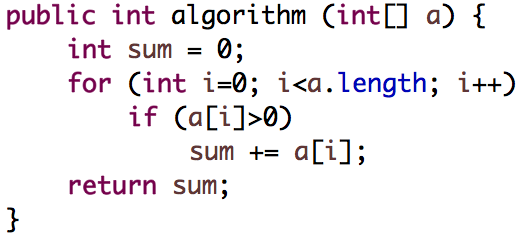
\includegraphics[height=4cm]{algorithm}

\begin{exampleblock}{Aufgabe}
	Wie viele \emph{Instruktionen} werden aufgerufen? \\% Worst-Case: n+1, Best-Case: 1, Average Case ?
	\pause
	Im \emph{worst case}? Im \emph{best case}? Im \emph{average case}?
\end{exampleblock}
\end{frame}

\subsection{O-Kalkül}
\begin{frame}{O-Notation}
	\begin{block}{Def. Asymptotisches Wachstum $\asymp$}
		Seien $f,g \from \nN_0 \to \Rnullplus$. Dann gilt
		\[
			f \asymp g \Leftrightarrow \exists c,c'\in \Rplus: \exists n_0\in \nN_0: \forall n\geq n_0: c f(n) \leq g(n) \leq c' f(n)
		\]
		Man sagt auch $g$ wächst genauso schnell wie $f$. $\asymp$ ist eine Äquivalenzrelation.
	\end{block}

	\begin{exampleblock}{Beispiele}
		\begin{itemize}
			\item $42n^6-33n^3+222n^2 -15 \asymp 66n^6+55555n^5$
			\item $n^{3+1}+5n^2\asymp 3n^3-n$
		\end{itemize}
	\end{exampleblock}
\end{frame}

\begin{frame}{$O$-Notation}
    \begin{block}{$\Theta$-Kalkül}
    	\begin{align*}
  			\Theta(f) &= \{ g \mid f \asymp g \} \\
  				   &= \{ g \mid \exists c,c'\in \Rplus: \exists n_0\in \nN_0: \forall  n\geq n_0: c f(n) \leq g(n) \leq c' f(n) \} 
		\end{align*}
    \end{block}

    \begin{exampleblock}{Bemerkungen}
    	\begin{itemize}
    		\item Im $\Theta$-Kalkül von $f(n)$ sind genau die Funktionen enthalten, die asymptotisch gleich schnell wachsen wie $f(n)$.
    		\item Schreibe $g(n) \in \Theta(f(n))$, wenn $g(n)$ asymptotisch gleichschnell wächst wie $f(n)$.
    		\item Ist $f$ ein Polynom, so sind insbesondere in $\Theta(f(n))$ alle Polynome enthalten, die den gleichen Grad wie $f$ haben.
    		\item Es gilt $\log_b(n) \in\Theta(\log_a(n))$. Die Basis ist also egal und man kann auch $\Theta(\log n)$ schreiben. % TODO Aufgabe und Beweis hierzu
    		% TODO Theta ist != Average Case
    	\end{itemize}
    \end{exampleblock}
\end{frame}

\begin{frame}{$O$-Notation}
    \begin{block}{Def.: $O$-Kalkül}
    	\[
    		O(f) = \{ g \mid \exists c\in \Rplus:\exists n_0\in\nN_0: \forall n\geq n_0: g(n) \leq c f(n)\}
    	\]

    	$g(n) \in O(f(n))$ (oder $g \preceq f$) genau dann, wenn $g$ asymptotisch höchstens so schnell wächst wie $f$.
    \end{block}
\pause
    \begin{block}{Def.: $\Omega$-Kalkül}
    	\[
    		\Omega(f) = \{ g \mid \exists c\in \Rplus:\exists n_0\in\nN_0: \forall n\geq n_0: g(n) \geq c f(n)\}
    	\]
    	
    	$g(n) \in \Omega(f(n))$ (oder $g \succeq f$) genau dann, wenn $g$ asymptotisch mindestens so schnell wächst wie $f$.
    \end{block}
\pause
    Beobachtung: $\Theta(f) = O(f) \cap \Omega(f)$
\end{frame}

\begin{frame}{$O$-Notation}
	\begin{exampleblock}{Aufgabe}
		\begin{enumerate}
			\item Für welches $c \in \Rplus$ gilt $5n^4 \in O(n^c)$ bzw $5n^4 \in \Omega(n^c)$?
			\item Für welches $c \in \Rplus$ gilt $5n^4 \in O(c^n)$ bzw $5n^4 \in \Omega(c^n)$?
			\item Für welches $c \in \Rplus$ gilt $2^n \in O(c^n)$ bzw $2^n \in \Omega(c^n)$?
			\item Zeige oder widerlege: $n \in \Theta(\sqrt{n})$
		\end{enumerate}
	\end{exampleblock}
\pause
	\begin{block}{Lösung}
		\begin{enumerate}
			\item Es gilt: $\forall c \geq 4$ bzw. $\forall c \leq 4$.
			\item Es gilt: $\forall c > 1$ bzw. $\forall c \leq 1$.
			\item Es gilt: $\forall c \geq 2$ bzw. $\forall c \leq 2$.
			\item \small Annahme: Die Behauptung ist richtig.\\
				Dann gilt: $n \in O(\sqrt{n}) \wedge n \in \Omega(\sqrt{n})$, insbesondere $n \in \Omega(\sqrt{n})$.\\
				$\Rightarrow \exists c\in \Rplus:\exists n_0\in\nN_0: \forall n\geq n_0: n \leq c \sqrt{n} \Leftrightarrow \frac{n}{\sqrt{n}} \leq c \Leftrightarrow \sqrt{n} \leq c$. Widerspruch.
				
		\end{enumerate}
	\end{block}
\end{frame}

\begin{frame}{$O$-Notation}
    \begin{exampleblock}{Aufgabe}
    	Zeige oder widerlege:
    	\[
    		f(n) + g(n) \in O(g(f(n)))
    	\]
    \end{exampleblock}
\pause
	\begin{block}{Lösung}
		Die Behauptung stimmt nicht. Wähle z.B. $f(n) = n^2$ und $g(n) = \sqrt{n}$ und führe dies zu einem Widerspruch.
	\end{block}
\end{frame}

\begin{frame}{$O$-Notation} % TODO: Logarithmusregeln, Typische Abschätzungskette (1 < log n < sqrt(n) < n < n log n < n c (c>1) < c^n < n!)
    \begin{itemize}
    	\item $\Theta$ entspricht \emph{nicht} dem average case.
    	\item $O(1)$ bedeutet konstante Laufzeit
    	\item Beachtet den \emph{Trick} mit den Limites\footnote{Ich weiß nicht, ob ihr den als Beweis in der Klausur oder auf dem Blättern verwenden dürft. Zur Kontrolle sollte man ihn aber kennen.}
        \item Es gilt mit Konstante $c \in \Rplus$ mit $c>1$
        \[
            1 \preceq \log n \preceq \sqrt{n} \preceq n \preceq n \log n \preceq n^c \preceq c^n \preceq n!
        \]
        %\nachgucken https://martin-thoma.com/die-landau-symbole/
    \end{itemize}
\end{frame}

\subsection{Master-Theorem}
\begin{frame}{Mastertheorem}
    \textbf{Problemstellung:}\\[1cm]    
    Gegeben sei eine \emph{rekursiv} definierte Funktion $T$.\\
    Frage: Welche Laufzeit hat $T$?\\[1cm]
    Beispiel:
    \[
    	T(n) = 8 T \left(\frac{n}{2} \right) + 1000n^2
    \]
    \\[1cm]\centering$\Rightarrow$ \emph{Mastertheorem}
\end{frame}

\begin{frame}{Mastertheorem}
    \begin{block}{Def.: Mastertheorem}
    	Seien $a\geq 1$ und $b>1$ Konstanten, $f \from \nN \to \Rnullplus$ und $T(n)$ eine Laufzeitfunktion der Form
    	\[
			T = a T\left(\frac{n}{b}\right) + f 
		\]
		Dann gilt nach dem \textbf{Mastertheorem}:
		\begin{itemize}
			\item \textbf{Fall 1:} \\ Wenn $f \in O(n^{\log_b a -\varepsilon})$ für ein $\varepsilon>0$ ist, dann ist $T\in \Theta(n^{\log_b a})$.
			\item \textbf{Fall 2:} \\ Wenn $f \in \Theta(n^{\log_b a})$ ist, dann ist $T\in \Theta(n^{\log_b a}\log n)$.
			\item\textbf{Fall 3:} \\  Wenn $f \in \Omega(n^{\log_b a +\varepsilon})$ für ein $\varepsilon>0$ ist, und wenn es eine Konstante $d$ gibt mit $0<d<1$, so dass für alle hinreichend großen $n$ gilt $af\left(\frac{n}{b}\right)\leq d f(n)$, dann ist $T\in \Theta(f)$.
		\end{itemize}
    \end{block}
\end{frame}

\begin{frame}{Mastertheorem}
    \begin{exampleblock}{Beispiel zum 1. Fall}
    	Sei $T(n) = 8 T \left(\frac{n}{2} \right) + 1000n^2$.
    	\begin{itemize}
    		\item Aus der Formel lässt sich ablesen:\\
    			$a=8$, $b=2$, $f(n)=1000n^2$
    		\item $n^{\log_b a}$ bestimmen:\\
    			$\log_b a = \log_2 8 = 3 \Rightarrow n^{\log_b a} = n^3$
    		\item $n^{\log_b a}$ mit $f(n)$ vergleichen: $1000n^2 \in O(n^3-\varepsilon)$?\\
    			Ja, für $\varepsilon = 1$ gilt $1000n^2 \in O(n^2)$.
    		\item Mit dem Mastertheorem folgt:\\
    			$T(n) = \Theta(n^3)$
    	\end{itemize}
    \end{exampleblock}
\end{frame}


\begin{frame}{Mastertheorem}
    \begin{exampleblock}{Beispiel zum 2. Fall}
    	Sei $T(n) = 2 T \left(\frac{n}{2} \right) + 10n$.
    	\begin{itemize}
    		\item Aus der Formel lässt sich ablesen:\\
    			$a=2$, $b=2$, $f(n)=10n$
    		\item $n^{\log_b a}$ bestimmen:\\
    			$\log_b a = \log_2 2 = 1 \Rightarrow n^{\log_b a} = n^1$
    		\item $n^{\log_b a}$ mit $f(n)$ vergleichen: $10n \in \Theta(n)$?\\
    			Ja!
    		\item Mit dem Mastertheorem folgt:\\
    			$T(n) = \Theta(n \log n)$
    	\end{itemize}
    \end{exampleblock}
\end{frame}



\begin{frame}{Mastertheorem}
    \begin{exampleblock}{Beispiel zum 3. Fall}
    	Sei $T(n) = 2 T \left(\frac{n}{2} \right) + n^2$.
    	\begin{itemize}
    		\item Aus der Formel lässt sich ablesen:\\
    			$a=2$, $b=2$, $f(n)=n^2$
    		\item $n^{\log_b a}$ bestimmen:\\
    			$\log_b a = \log_2 2 = 1 \Rightarrow n^{\log_b a} = n^1$
    		\item $n^{\log_b a}$ mit $f(n)$ vergleichen: $n^2 \in \Omega(n^{1+\varepsilon})$?\\
    			Ja, für $\varepsilon = 1$ gilt $n^2 \in \Omega(n^2)$.
    		\item Zusatzbedingung überprüfen: Ist $af\left(\frac{n}{b}\right)\leq d f(n)$?\\
    			Ja, für $d = \frac{1}{2}$ gilt $\forall n \geq 1 \; : \; \frac{1}{2}n^2 \leq \frac{1}{2}n^2$
    		\item Mit dem Mastertheorem folgt:\\
    			$T(n) = \Theta(n^2)$
    	\end{itemize}
    \end{exampleblock}
\end{frame}

\section{Endliche Automaten}
\def\mybox#1{\hbox{\vrule height 2ex width 0pt depth 0.6ex#1}}
\def\taste[#1]#2{%
  \tikz[x=8mm,y=8mm,baseline=(N.base)] \tasteinnerx[#1]{#2};%
}
\def\tasteinnerx[#1]#2{%
  \node[midway,inner sep=0mm,draw,rounded corners,anchor=base,minimum width=10mm,#1] (N) {\mybox{#2}}%
}
\def\tasteinner[#1]#2{%
  node[midway,inner sep=0mm,draw,rounded corners,minimum width=10mm,#1] (N) {\mybox{#2}}%
}
\def\tasteinnerOK{\tasteinner[fill=green!20]{OK}}
\def\tasteOK{\taste[fill=green!20]{OK}}
\def\tasteC{\taste[fill=red!20]{C}}
\def\tasteinnerC{\tasteinner[fill=red!20]{C}}
\def\tasteRein{\taste[fill=blue!10]{rein}}
\def\tasteinnerRein{\tasteinner[fill=blue!10]{rein}}
\def\tasteZitro{\taste[fill=yellow!10]{zitro}}
\def\tasteinnerZitro{\tasteinner[fill=yellow!10]{zitro}}

\newcommand{\ioeps}[1]{#1|\varepsilon}

\subsection{Mealy-Automat}
\begin{frame}{Der Getränkeautomat}

	\begin{exampleblock}{Beispiel} \small
		Betrachte einen Getränkeautomaten:
		Man kann nur 1-Euro"=Stücke einwerfen und vier Tasten drücken: Es gibt
		zwei Auswahltasten für Mineralwasser \tasteRein{} und Zitronensprudel
		\tasteZitro{}, eine Abbruch"=Taste \tasteC{} und eine \tasteOK-Taste.

	
	\begin{itemize}
	\item Jede Flasche Sprudel kostet 1 Euro.
	\item Es kann ein Guthaben von 1 Euro gespeichert werden. Wirft man
	  weitere Euro"=Stücke ein, werden sie sofort wieder ausgegeben.
	\item Wenn man mehrfach Auswahltasten drückt, wird der letzte Wunsch
	  gespeichert.
	\item Bei Drücken der Abbruch"=Taste wird alles bereits eingeworfenen
	  Geld wieder zurückgegeben und kein Getränkewunsch mehr gespeichert.
	\item Drücken der OK-Taste wird ignoriert, solange noch kein Euro
	  eingeworfen wurde oder keine Getränkesorte ausgewählt wurde.

	  Andernfalls wird das gewünschte Getränk ausgeworfen.
	\end{itemize} 
	\end{exampleblock}
\end{frame}

\begin{frame}{Der Getränkeautomat}

	\begin{exampleblock}{Beispiel}
		\begin{figure}[ht]
  \centering
  \begin{tikzpicture}[x=8mm,y=8mm]
    % Rahmen
    \draw (0,0) -- (8,0) -- (8,8) .. controls  (3,9) and (5,9) .. (0,8) -- cycle;
    % Geldschlitz 
    \draw (1.4,5.5) rectangle ++(0.2,1) ++(-0.1,0) node[anchor=south] {\vbox{\hbox{Geld-}\hbox{Einwurf}}};
    % Geldrückgabe 
    \draw (1,1) rectangle ++(1,1) ++(-0.5,0) node[anchor=south] {\vbox{\hbox{Geld-}\hbox{Rückgabe}}};
    % Warenauswurf
    \draw (4,1) rectangle ++(3.5,1) ++(-1.75,0) node[anchor=south] {Ware};
    
    % Tasten
    \draw (2.75,3) ++(3,3.5) node[anchor=south] {Sprudel};
    \draw (4,5.5) rectangle ++(1.5,1)\tasteinnerRein;
    \draw (6,5.5) rectangle ++(1.5,1) \tasteinnerZitro;
    \draw (4,4) rectangle ++(1.5,1) \tasteinnerOK;
    \draw (6,4) rectangle ++(1.5,1) \tasteinnerC;
  \end{tikzpicture}
  \caption{Ein primitiver Getr"ankeautomat}
  \label{fig:getraenkeautomat}
\end{figure}
	\end{exampleblock}
\end{frame}

\begin{frame}[fragile]{Der Getränkeautomat}

	\begin{exampleblock}{Beispiel}
		\begin{figure}[ht]
  \centering
  \small
  \begin{tikzpicture}[->,>=stealth]
    \matrix[matrix of math nodes,column sep=25mm,row sep=20mm,nodes={circle,draw,inner sep=1pt}]   {
      |(0-)| (0,-) & |(0R)| (0,R) & |(0Z)| (0,Z) \\
      |(1-)| (1,-) & |(1R)| (1,R) & |(1Z)| (1,Z) \\
    };

    \coordinate[left of=0-] (start);

    \draw (start) -- node[auto] {} (0-);

    % Schleifen
    \draw (0-) edge[loop above]  node[pos=0.5] {$\ioeps{O}$,$\ioeps{C}$} ();
    \draw (0R) edge[loop above] node[pos=0.9,anchor=west] {$\ioeps{R}$,$\ioeps{O}$} ();
    \draw (0Z) edge[loop above] node[pos=0.5] {$\ioeps{Z}$,$\ioeps{O}$} ();
    \draw (1-) edge[loop below]  node[pos=0.5] {$\io{1}{1}$,$\ioeps{O}$} ();
    \draw (1R) edge[loop below] node[pos=0.9,anchor=east] {$\io{1}{1}$,$\ioeps{R}$} ();
    \draw (1Z) edge[loop below] node[pos=0.5] {$\io{1}{1}$,$\ioeps{Z}$} ();

    % andere Kanten
    \draw (0-) -- node[right,pos=0.2] {$\ioeps{1}$} (1-);
    \draw (0R) -- node[right,pos=0.2] {$\ioeps{1}$} (1R);
    \draw (0Z) -- node[right,pos=0.2] {$\ioeps{1}$} (1Z);

    \draw (1-) to[bend left=10] node[left,pos=0.2] {$\io{C}{1}$} (0-);

    \draw (0-) to[bend right=10] node[below] {$\ioeps{R}$} (0R);
    \draw (0R) to[bend right=10] node[above,pos=0.1] {$\ioeps{C}$} (0-);
    \draw (0R) to[bend right=10] node[below] {$\ioeps{Z}$} (0Z);
    \draw (0Z) to[bend right=10] node[above] {$\ioeps{R}$} (0R);
    \draw (0-) to[bend left=32]  node[below,pos=0.2] {$\ioeps{Z}$} (0Z);
    \draw (0Z) to[bend right=40] node[above] {$\ioeps{C}$} (0-);

    \draw (1-) to[bend right=10] node[above] {$\ioeps{R}$} (1R);
    \draw (1R) -- node[below,pos=0.4,anchor=north east] {$\io{O}{R}$,$\io{C}{1}$} (0-); %!!
    \draw (1R) to[bend right=10] node[below] {$\ioeps{Z}$} (1Z);
    \draw (1Z) to[bend right=10] node[above] {$\ioeps{R}$} (1R);
    \draw (1-) to[bend left=-32] node[below,pos=0.2] {$\ioeps{Z}$} (1Z);
    \draw (1Z) -- node[above,pos=0.3,anchor=south west] {$\io{O}{Z}$,$\io{C}{1}$} (0-); %!!
  \end{tikzpicture}
\end{figure}
	\end{exampleblock}
\end{frame}

\begin{frame}{Mealy-Automat}
	\begin{block}{Def.: Mealy-Automat}
		Ein (endlicher) \textbf{Mealy-Automat} $A=(Z, z_0, X, f, Y, g)$ ist bestimmt durch:
		\begin{itemize}
			\item endliche Zustandsmenge $Z$,
			\item Anfangszustand $z_0 \in Z$,
			\item Eingabealphabet $X$,
			\item Zustandsüberführungsfunktion $f: Z \times X \rightarrow Z$,
			\item Ausgabealphabet $Y$,
			\item Ausgabefunktion $g: Z \times X \rightarrow Y^{\ast}$
		\end{itemize}
	\end{block}
\pause
	\begin{alertblock}{Achtung!}
	$f$ ist eine \textbf{Funktion}, also muss man von jedem Zustand mit allen Eingaben ``irgendwohin'' gelangen! Stichwort: Müllzustand.
	\end{alertblock}
\end{frame}



\begin{frame}{Mealy-Automat}
	\begin{block}{Def.: Verallgemeinerte Zustandsübergangsfunktion $f_{\ast}$}
		$f_{\ast} : Z \times X^{\ast} \rightarrow Z$ gibt den Zustand aus, der durch die Eingabe eines Wortes erreicht wird, und ist definiert durch:
		\begin{align*}
			f_{\ast}(z,\varepsilon) &= z \\
			\forall w \in X^{\ast} : \forall x \in X : f_{\ast}(z,wx) &= f(f_{\ast}(z,w),x)\\
		\end{align*}
		Oder als alternative Definition:
		\begin{align*}
			\bar{f}_{\ast}(z,\varepsilon) &= z \\
			\forall w \in X^{\ast} : \forall x \in X : \bar{f}_{\ast}(z,xw) &= \bar{f}_{\ast}(f(z,x),w)
		\end{align*}
	\end{block}
\end{frame}

\begin{frame}{Mealy-Automat}
	\begin{block}{Def.: Verallgemeinerte Zustandsübergangsfunktion $f_{\ast\ast}$}
		$f_{\ast\ast} : Z \times X^{\ast} \rightarrow Z^{\ast}$ gibt \textbf{alle} Zustände aus, die bei der Eingabe eines Wortes durchlaufen werden, und ist definiert durch:
		\begin{align*}
			f_{\ast\ast}(z,\varepsilon) = z\\
			\forall w \in X^{\ast} : \forall x \in X : f_{\ast\ast}(z,wx) &= f_{\ast\ast}(z,w) \cdot f(f_{\ast}(z,w),x)\\
		\end{align*}
	\end{block}
\end{frame}

\begin{frame}[fragile]{Mealy-Automat}

	\begin{exampleblock}{Aufgabe zu $f_{\ast}$ und $f_{\ast\ast}$}
		\begin{columns}
			\begin{column}{0.6\textwidth}
				\begin{figure}[ht]
  \centering
  \tiny
  \begin{tikzpicture}[->,>=stealth]
    \matrix[matrix of math nodes,column sep=20mm,row sep=20mm,nodes={circle,draw,inner sep=1pt}]   {
      |(0-)| (0,-) & |(0R)| (0,R) & |(0Z)| (0,Z) \\
      |(1-)| (1,-) & |(1R)| (1,R) & |(1Z)| (1,Z) \\
    };

    \coordinate[left of=0-] (start);

    \draw (start) -- node[auto] {} (0-);

    % Schleifen
    \draw (0-) edge[loop above]  node[pos=0.5] {$\ioeps{O}$,$\ioeps{C}$} ();
    \draw (0R) edge[loop above] node[pos=0.9,anchor=west] {$\ioeps{R}$,$\ioeps{O}$} ();
    \draw (0Z) edge[loop above] node[pos=0.5] {$\ioeps{Z}$,$\ioeps{O}$} ();
    \draw (1-) edge[loop below]  node[pos=0.5] {$\io{1}{1}$,$\ioeps{O}$} ();
    \draw (1R) edge[loop below] node[pos=0.9,anchor=east] {$\io{1}{1}$,$\ioeps{R}$} ();
    \draw (1Z) edge[loop below] node[pos=0.5] {$\io{1}{1}$,$\ioeps{Z}$} ();

    % andere Kanten
    \draw (0-) -- node[right,pos=0.2] {$\ioeps{1}$} (1-);
    \draw (0R) -- node[right,pos=0.2] {$\ioeps{1}$} (1R);
    \draw (0Z) -- node[right,pos=0.2] {$\ioeps{1}$} (1Z);

    \draw (1-) to[bend left=10] node[left,pos=0.2] {$\io{C}{1}$} (0-);

    \draw (0-) to[bend right=10] node[below] {$\ioeps{R}$} (0R);
    \draw (0R) to[bend right=10] node[above,pos=0.1] {$\ioeps{C}$} (0-);
    \draw (0R) to[bend right=10] node[below] {$\ioeps{Z}$} (0Z);
    \draw (0Z) to[bend right=10] node[above] {$\ioeps{R}$} (0R);
    \draw (0-) to[bend left=32]  node[below,pos=0.2] {$\ioeps{Z}$} (0Z);
    \draw (0Z) to[bend right=40] node[above] {$\ioeps{C}$} (0-);

    \draw (1-) to[bend right=10] node[above] {$\ioeps{R}$} (1R);
    \draw (1R) -- node[below,pos=0.4,anchor=north east] {$\io{O}{R}$,$\io{C}{1}$} (0-); %!!
    \draw (1R) to[bend right=10] node[below] {$\ioeps{Z}$} (1Z);
    \draw (1Z) to[bend right=10] node[above] {$\ioeps{R}$} (1R);
    \draw (1-) to[bend left=-32] node[below,pos=0.2] {$\ioeps{Z}$} (1Z);
    \draw (1Z) -- node[above,pos=0.3,anchor=south west] {$\io{O}{Z}$,$\io{C}{1}$} (0-); %!!
  \end{tikzpicture}
\end{figure}
			\end{column}
			\begin{column}{0.375\textwidth}
			\small
				Gib an:
				\begin{enumerate}
					\item $f_{\ast}((0,-), R1O)$
					\item $f_{\ast\ast}((0,-), R1O)$
					\item $f_{\ast}((0,-), C1Z)$
					\item $f_{\ast\ast}((0,-), RZO)$
					\item $f_{\ast\ast}((1,Z), RZO)$
					\item $f_{\ast}((0,-), RZ1R1C1ZO)$
				\end{enumerate}
			\end{column}
		\end{columns}
	\end{exampleblock}
\end{frame}

\begin{frame}{Mealy-Automat}
	\begin{block}{Lösung zur Aufgabe zu $f_{\ast}$ und $f_{\ast\ast}$}
		\begin{enumerate}
					\item $f_{\ast}((0,-), R1O) = (0,-)$
					\item $f_{\ast\ast}((0,-), R1O) = (0,-)(0,R)(1,R)(0,-)$
					\item $f_{\ast}((0,-), C1Z) = (1,Z)$
					\item $f_{\ast\ast}((0,-), RZO) = (0,-)(0,R)(0,Z)(0,Z)$
					\item $f_{\ast\ast}((1,Z), RZO) = (1,Z)(1,R)(1,Z)(0,-)$
					\item $f_{\ast}((0,-), RZ1R1C1ZO)= (0,-)$
				\end{enumerate}
	\end{block}
\end{frame}

\begin{frame}{Mealy-Automat}
	\begin{block}{Def.: Verallgemeinerte Ausgabefunktion $g_{\ast}$}
		$g_{\ast} : Z \times X^{\ast} \rightarrow Z$ gibt die letzte Ausgabe aus, die durch die Eingabe eines Wortes produziert wird, und ist definiert durch:
		\begin{align*}
			g_{\ast}(z,\varepsilon) &= \varepsilon \\
			\forall w \in X^{\ast} : \forall x \in X : g_{\ast}(z,wx) &= g(f_{\ast}(z,w),x)\\
		\end{align*}
	\end{block}

	\begin{block}{Def.: Verallgemeinerte Ausgabefunktion $g_{\ast\ast}$}
		$g_{\ast\ast} : Z \times X^{\ast} \rightarrow Z^{\ast}$ gibt \textbf{alle} Ausgaben konkateniert aus, die bei der Eingabe eines Wortes erzeugt werden, und ist definiert durch:
		\begin{align*}
			g_{\ast\ast}(z,\varepsilon) = \varepsilon\\
			\forall w \in X^{\ast} : \forall x \in X : g_{\ast\ast}(z,wx) &= g_{\ast\ast}(z,w) \cdot g_{\ast}(z,wx)\\
		\end{align*}
	\end{block}
\end{frame}

\begin{frame}[fragile]{Mealy-Automat}

	\begin{exampleblock}{Aufgabe zu $g_{\ast}$ und $g_{\ast\ast}$}
		\begin{columns}
			\begin{column}{0.6\textwidth}
				\begin{figure}[ht]
  \centering
  \tiny
  \begin{tikzpicture}[->,>=stealth]
    \matrix[matrix of math nodes,column sep=20mm,row sep=20mm,nodes={circle,draw,inner sep=1pt}]   {
      |(0-)| (0,-) & |(0R)| (0,R) & |(0Z)| (0,Z) \\
      |(1-)| (1,-) & |(1R)| (1,R) & |(1Z)| (1,Z) \\
    };

    \coordinate[left of=0-] (start);

    \draw (start) -- node[auto] {} (0-);

    % Schleifen
    \draw (0-) edge[loop above]  node[pos=0.5] {$\ioeps{O}$,$\ioeps{C}$} ();
    \draw (0R) edge[loop above] node[pos=0.9,anchor=west] {$\ioeps{R}$,$\ioeps{O}$} ();
    \draw (0Z) edge[loop above] node[pos=0.5] {$\ioeps{Z}$,$\ioeps{O}$} ();
    \draw (1-) edge[loop below]  node[pos=0.5] {$\io{1}{1}$,$\ioeps{O}$} ();
    \draw (1R) edge[loop below] node[pos=0.9,anchor=east] {$\io{1}{1}$,$\ioeps{R}$} ();
    \draw (1Z) edge[loop below] node[pos=0.5] {$\io{1}{1}$,$\ioeps{Z}$} ();

    % andere Kanten
    \draw (0-) -- node[right,pos=0.2] {$\ioeps{1}$} (1-);
    \draw (0R) -- node[right,pos=0.2] {$\ioeps{1}$} (1R);
    \draw (0Z) -- node[right,pos=0.2] {$\ioeps{1}$} (1Z);

    \draw (1-) to[bend left=10] node[left,pos=0.2] {$\io{C}{1}$} (0-);

    \draw (0-) to[bend right=10] node[below] {$\ioeps{R}$} (0R);
    \draw (0R) to[bend right=10] node[above,pos=0.1] {$\ioeps{C}$} (0-);
    \draw (0R) to[bend right=10] node[below] {$\ioeps{Z}$} (0Z);
    \draw (0Z) to[bend right=10] node[above] {$\ioeps{R}$} (0R);
    \draw (0-) to[bend left=32]  node[below,pos=0.2] {$\ioeps{Z}$} (0Z);
    \draw (0Z) to[bend right=40] node[above] {$\ioeps{C}$} (0-);

    \draw (1-) to[bend right=10] node[above] {$\ioeps{R}$} (1R);
    \draw (1R) -- node[below,pos=0.4,anchor=north east] {$\io{O}{R}$,$\io{C}{1}$} (0-); %!!
    \draw (1R) to[bend right=10] node[below] {$\ioeps{Z}$} (1Z);
    \draw (1Z) to[bend right=10] node[above] {$\ioeps{R}$} (1R);
    \draw (1-) to[bend left=-32] node[below,pos=0.2] {$\ioeps{Z}$} (1Z);
    \draw (1Z) -- node[above,pos=0.3,anchor=south west] {$\io{O}{Z}$,$\io{C}{1}$} (0-); %!!
  \end{tikzpicture}
\end{figure}
			\end{column}
			\begin{column}{0.4\textwidth}
			\small
				Gib an:
				\begin{enumerate}
					\item $g_{\ast}((0,-), R1O)$
					\item $g_{\ast\ast}((0,-), R1O)$
					\item $g_{\ast\ast}((0,-), R11O)$
					\item $g_{\ast}((0,-), C1Z)$
					\item $g_{\ast\ast}((0,-), RZO)$
					\item $g_{\ast\ast}((1,Z), RZO)$
					\item $g_{\ast\ast}((0,-), RZ1R1C1ZO)$
				\end{enumerate}
			\end{column}
		\end{columns}
	\end{exampleblock}
\end{frame}

\begin{frame}{Mealy-Automat}
	\begin{block}{Lösung zur Aufgabe zu $g_{\ast}$ und $g_{\ast\ast}$}
		\begin{enumerate}
					\item $g_{\ast}((0,-), R1O) = R$
					\item $g_{\ast\ast}((0,-), R1O) = R$
					\item $g_{\ast\ast}((0,-), R11O) = 1R$
					\item $g_{\ast}((0,-), C1Z) = \varepsilon$
					\item $g_{\ast\ast}((0,-), RZO) = \varepsilon$
					\item $g_{\ast\ast}((1,Z), RZO) = Z $
					\item $g_{\ast\ast}((0,-), RZ1R1C1ZO)= 11Z$
				\end{enumerate}
	\end{block}
\end{frame}



\subsection{Moore-Automat}
\begin{frame}{Moore-Automat}
	\begin{block}{Def.: Moore-Automat}
		Ein (endlicher) \textbf{Moore-Automat} $A=(Z, z_0, X, f, Y, h)$ ist bestimmt durch:
		\begin{itemize}
			\item endliche Zustandsmenge $Z$,
			\item Anfangszustand $z_0 \in Z$,
			\item Eingabealphabet $X$,
			\item Zustandsüberführungsfunktion $f: Z \times X \rightarrow Z$,
			\item Ausgabealphabet $Y$,
			\item Ausgabefunktion $h: Z \rightarrow Y^{\ast}$
		\end{itemize}

	Der Unterschied zum Mealy Automaten ist also , dass die Ausgabe nur vom Zustand abhängt, nicht von der Eingabe.

	\end{block}
\end{frame}

\begin{frame}[fragile]{Moore-Automat}
	\begin{exampleblock}{Beispiel}
		\begin{figure}[ht]
  \centering
  \begin{tikzpicture}[shorten >=1pt,node distance=2cm,auto,initial text=,->,>=stealth]
   \node[state,initial]  (q_0)                       {$q_{\varepsilon}\!\mid\! 0$};
   \node[state]          (q_1) [above right of= q_0] {$q_{a}\!\mid\! 0$};
    \node[state]          (q_2) [below right of= q_0] {$q_{b}\!\mid\! 0$};
   \node[state](q_3) [below right of=q_1] {$q_f\!\mid\! 1$};
   \node[state](q_4) [right of=q_3] {$q_r\!\mid\! 0$};
    \path[->] (q_0) edge              node        {$a$} (q_1)
                    edge              node [swap] {$b$} (q_2)
              (q_1) edge              node        {$b$} (q_3)
                    edge [loop above] node        {$a$} ()
              (q_2) edge              node [swap] {$a$} (q_3)
                    edge [loop below] node        {$b$} ()
              (q_3) edge              node        {$a,b$} (q_4)
              (q_4) edge [loop above] node        {$a,b$} ();
  \end{tikzpicture}
\end{figure}
	\end{exampleblock}
\end{frame}

\begin{frame}{Moore-Automat}
	\begin{block}{Def.: Verallgemeinerte Zustandsübergangsfunktionen $f_{\ast}$ und $f_{\ast\ast}$}
		Wie bei Mealy-Automaten.
	\end{block}

	\begin{block}{Def.: Verallgemeinerte Ausgabenfunktion $g_{\ast} = h \circ f_{\ast}$}
		$g_{\ast} : Z \times X^{\ast} \rightarrow Y$ gibt die letzte Ausgabe aus und ist definiert durch:
		\[
			\forall(z,w) \in Z \times X^{\ast} : g_{\ast}(z,w) = h(f_{\ast}(z,w))
		\]
	\end{block}

	\begin{block}{Def.: Verallgemeinerte Ausgabenfunktion $g_{\ast\ast} = h^{\ast\ast} \circ f_{\ast\ast}$}
		$g_{\ast\ast} : Z \times X^{\ast} \rightarrow Y$ gibt alle Ausgaben konkateniert aus und ist definiert durch:
		\[
			\forall(z,w) \in Z \times X^{\ast} : g_{\ast\ast}(z,w) = h^{\ast\ast}(f_{\ast\ast}(z,w))
		\]
		mit $h^{\ast\ast} :$\textit{induzierter Homomorphismus von h}.
	\end{block}
\end{frame}

\begin{frame}[fragile]{Moore-Automat}

	\begin{exampleblock}{Aufgabe zu $f_{\ast}$, $f_{\ast\ast}$, $g_{\ast}$ und $g_{\ast\ast}$}
		\begin{columns}
			\begin{column}{0.6\textwidth}
				\begin{figure}[ht]
  \centering
  \small
  \begin{tikzpicture}[shorten >=1pt,node distance=2cm,auto,initial text=,->,>=stealth]
   \node[state,initial]  (q_0)                       {$q_{\varepsilon}\!\mid\! 0$};
   \node[state]          (q_1) [above right of= q_0] {$q_{a}\!\mid\! 0$};
    \node[state]          (q_2) [below right of= q_0] {$q_{b}\!\mid\! 0$};
   \node[state](q_3) [below right of=q_1] {$q_f\!\mid\! 1$};
   \node[state](q_4) [right of=q_3] {$q_r\!\mid\! 0$};
    \path[->] (q_0) edge              node        {$a$} (q_1)
                    edge              node [swap] {$b$} (q_2)
              (q_1) edge              node        {$b$} (q_3)
                    edge [loop above] node        {$a$} ()
              (q_2) edge              node [swap] {$a$} (q_3)
                    edge [loop below] node        {$b$} ()
              (q_3) edge              node        {$a,b$} (q_4)
              (q_4) edge [loop above] node        {$a,b$} ();
  \end{tikzpicture}
\end{figure}
			\end{column}
			\begin{column}{0.4\textwidth}
			\small
				Gib an:
				\begin{enumerate}
					\item $f_{\ast}(q_{\varepsilon}, aab)$
					\item $f_{\ast\ast}(q_{\varepsilon}, aab)$

					\item $g_{\ast}(q_{\varepsilon}, aab)$
					\item $g_{\ast\ast}(q_{\varepsilon}, aab)$
					\item $g_{\ast}(q_{\varepsilon}, abab)$
					\item $g_{\ast\ast}(q_{f}, abab)$
				\end{enumerate}
			\end{column}
		\end{columns}
	\end{exampleblock}
\end{frame}

\begin{frame}{Moore-Automat}
	\begin{block}{Lösung zur Aufgabe zu $f_{\ast}$, $f_{\ast\ast}$, $g_{\ast}$ und $g_{\ast\ast}$}
		\begin{enumerate}
					\item $f_{\ast}(q_{\varepsilon}, aab) = q_{f}$
					\item $f_{\ast\ast}(q_{\varepsilon}, aab) = q_{\varepsilon}q_{a}q_{a}q_{f}$

					\item $g_{\ast}(q_{\varepsilon}, aab) = 1$
					\item $g_{\ast\ast}(q_{\varepsilon}, aab) = 0001$
					\item $g_{\ast}(q_{\varepsilon}, abab) = 0$
					\item $g_{\ast\ast}(q_{f}, abba) = 10000$
			\end{enumerate}
	\end{block}
\end{frame}

\subsection{Akzeptoren}
\begin{frame}{Endlicher Akzeptor}
	\begin{block}{Def.: Endlicher Akzeptor}
		Ein \textbf{endlicher Akzeptor} ist eine Spezialform des Moore-Automaten mit immer genau einem Bit Ausgabe, d.h. $Y = \set{0,1}$ (und $\forall z : h(z) \in Y$).

		Man definiert deshalb eine Menge $F = \setc{z}{h(z)=1}$ der \textbf{akzeptierenden Zustände}.

		Ein endlicher Akzeptor ist also definiert durch:

		\begin{itemize}
			\item endliche Zustandsmenge $Z$,
			\item Anfangszustand $z_0 \in Z$,
			\item Eingabealphabet $X$,
			\item Zustandsüberführungsfunktion $f: Z \times X \rightarrow Z$,
			\item eine Menge akzeptierender Zustände $F \subseteq Z$
		\end{itemize}
		Die von einem endlichen Akzeptor $A$ \textbf{akzeptierte Sprache} ist:
		\[
			L(A) = \setc{w \in X^{\ast}}{f_{\ast}(z_{0},w) \in F}
		\]
	\end{block}
\end{frame}

\begin{frame}[fragile]{Endlicher Akzeptor}
	\begin{exampleblock}{Beispiel}
	\begin{columns}
		\begin{column}{0.6\textwidth}
		\begin{figure}[ht]
  \centering
  \begin{tikzpicture}[shorten >=1pt,node distance=2cm,auto,initial text=,->,>=stealth]
    \node[state,initial]  (q_0)                       {$q_{\varepsilon}$};
    \node[state]          (q_1) [above right of= q_0] {$q_{a}$};
    \node[state]          (q_2) [below right of= q_0] {$q_{b}$};
    \node[state,accepting](q_3) [below right of=q_1] {$q_f$};
    \node[state](q_4) [right of=q_3] {$q_r$};
    \path[->] (q_0) edge              node        {$a$} (q_1)
                    edge              node [swap] {$b$} (q_2)
              (q_1) edge              node        {$b$} (q_3)
                    edge [loop above] node        {$a$} ()
              (q_2) edge              node [swap] {$a$} (q_3)
                    edge [loop below] node        {$b$} ()
              (q_3) edge              node        {$a,b$} (q_4)
              (q_4) edge [loop above] node        {$a,b$} ();
  \end{tikzpicture}
\end{figure}		
		\end{column}
		\begin{column}{0.375\textwidth}
		\centering
		(Akzeptierende Zustände mit Doppelkringel)
		\begin{figure}[ht]
			\begin{tikzpicture}[shorten >=1pt,node distance=2cm,auto,initial text=,->,>=stealth]
				\node[state,accepting] (z) {$z$};
			\end{tikzpicture}
		\end{figure}
		\end{column}
		
	\end{columns}
	\end{exampleblock}
\end{frame}

\begin{frame}{Endlicher Akzeptor}
	\begin{exampleblock}{Aufgabe zu endlichen Akzeptoren}
		\begin{enumerate}
			\small
			\item Zeichne einen Akzeptor mit $X=\set{a,b}$, der alle Wörter akzeptiert, bei denen die Anzahl der \emph{a} durch 5 teilbar ist.
			\item Zeichne einen Akzeptor mit $X=\set{a,b}$, der alle Wörter akzeptiert, in denen nirgends hintereinander zwei \emph{b} vorkommen.
			\item Zeichne einen Akzeptor mit $X=\set{a,b}$, der alle Wörter akzeptiert, in denen irgendwo das Teilwort \emph{abab} vorkommt.
			\item Zeichne einen Akzeptor mit $X=\set{a,b}$, der alle Wörter akzeptiert, in denen nirgends das Teilwort \emph{abab} vorkommt.
			\item Welche Sprache wird vom folgenden Akzeptor $A$ erkannt?
		\end{enumerate}

		\begin{figure}[ht]
  			\centering
  			\begin{tikzpicture}[shorten >=1pt,node distance=2cm,auto,initial text=,->,>=stealth]
   			 	\node[state,initial]  (s_0)                       {$s_{0}$};
  			 	\node[state,accepting](s_1) [right of= s_0] {$s_{1}$};
  			 	\node[state]          (s_2) [right of= s_1] {$s_{2}$};
    			\node[state,accepting](s_3) [right of= s_2] {$s_3$};
    			\draw[->] 	(s_0) 	edge              	node        {$a,b$} (s_1);
              	\draw[->]	(s_1) 	to [bend left=20] 	node        {$a,b$} (s_2);
              	\draw[->]	(s_2) 	to [bend left=20] 	node 		{$b$} 	(s_3);
              	\draw[->]	(s_2)	to [bend left=20] 	node 		{$a$} 	(s_1);
              	\draw[->]	(s_3)	to [bend left=20] 	node 		{$a,b$} (s_2);
  \end{tikzpicture}
\end{figure}	
	\end{exampleblock}
\end{frame}

\begin{frame}{Endlicher Akzeptor}

	\begin{block}{Lösung zur Aufgabe zu endlichen Akzeptoren}
		\begin{enumerate}
			\item siehe Tafel
		\item siehe Tafel
		\item siehe Tafel
		\item siehe Tafel
		\item $L(A)= \setc{w \in \set{a,b}^{\ast}}{\,\setsize{w} mod\, 2 = 1} = \setC{w \in \set{a,b}^{\ast}}{$w$ hat ungerade Länge}$
		\end{enumerate}		
	\end{block}
\end{frame}

\begin{frame}{Endlicher Akzeptor}

	\begin{block}{Lösung}

	1. Zeichne einen Akzeptor mit $X=\set{a,b}$, der alle Wörter akzeptiert, bei denen die Anzahl der \emph{a} durch 5 teilbar ist.\\

	\textbf{Lösung:}\\

	\centering \begin{tikzpicture}[shorten >=1pt,node distance=2cm,auto,initial text=,->,>=stealth]
   		\node[state,initial, accepting] (s_0) {$s_{0}$};
  		\node[state] (s_1) [right of= s_0] {$s_{1}$};
  		\node[state] (s_2) [right of= s_1] {$s_{2}$};
    	\node[state] (s_3) [right of= s_2] {$s_3$};
    	\node[state] (s_4) [right of= s_3] {$s_4$};
    	\draw[->] (s_0) edge node {$a$} (s_1);
    	\draw[->] (s_1) edge node {$a$} (s_2);
    	\draw[->] (s_2) edge node {$a$} (s_3);
    	\draw[->] (s_3) edge node {$a$} (s_4);
    	\draw[->] (s_0) edge node {$a$} (s_1);
    	\draw[->] (s_0) to [loop above] node {$b$} (s_0);
    	\draw[->] (s_1) to [loop above] node {$b$} (s_1);
    	\draw[->] (s_2) to [loop above] node {$b$} (s_2);
    	\draw[->] (s_3) to [loop above] node {$b$} (s_3);
    	\draw[->] (s_4) to [loop above] node {$b$} (s_4);
    	\draw[->] (s_4) to [bend left] node {$b$} (s_0);
 	\end{tikzpicture}
	\end{block}
\end{frame}

\begin{frame}{Endlicher Akzeptor}

	\begin{block}{Lösung}

	2. Zeichne einen Akzeptor mit $X=\set{a,b}$, der alle Wörter akzeptiert, in denen nirgends hintereinander zwei \emph{b} vorkommen.\\

	\textbf{Lösung:}\\

	\centering \begin{tikzpicture}[shorten >=1pt,node distance=2cm,auto,initial text=,->,>=stealth]
   		\node[state,initial,accepting] (s_0) {$s_{0}$};
  		\node[state,accepting] (s_1) [right of= s_0] {$s_{1}$};
  		\node[state] (s_2) [right of= s_1] {$s_{2}$};
    	\draw[->] (s_0) to [bend left] node {$b$} (s_1);
    	\draw[->] (s_1) to [bend left] node {$a$} (s_0);
    	\draw[->] (s_1) edge node {$b$} (s_2);
    	\draw[->] (s_0) to [loop above] node {$a$} (s_0);
    	\draw[->] (s_2) to [loop above] node {$a,b$} (s_2);
 	\end{tikzpicture}
	\end{block}
\end{frame}

\begin{frame}{Endlicher Akzeptor}

	\begin{block}{Lösung}

	3. Zeichne einen Akzeptor mit $X=\set{a,b}$, der alle Wörter akzeptiert, in denen irgendwo das Teilwort \emph{abab} vorkommt.\\

	\textbf{Lösung:}\\

	\centering \begin{tikzpicture}[shorten >=1pt,node distance=2cm,auto,initial text=,->,>=stealth]
   		\node[state,initial] (s_0) {$s_{0}$};
  		\node[state] (s_1) [right of= s_0] {$s_{1}$};
  		\node[state] (s_2) [right of= s_1] {$s_{2}$};
    	\node[state] (s_3) [right of= s_2] {$s_3$};
    	\node[state,accepting] (s_4) [right of= s_3] {$s_4$};

    	\draw[->] (s_0) edge node {$a$} (s_1);
    	\draw[->] (s_1) edge node {$b$} (s_2);
    	\draw[->] (s_2) edge node {$a$} (s_3);
    	\draw[->] (s_3) edge node {$b$} (s_4);

    	\draw[->] (s_2) to [bend left] node {$b$} (s_0);
    	\draw[->] (s_3) to [bend right] node[above] {$a$} (s_1);

    	\draw[->] (s_0) to [loop above] node {$b$} (s_0);
    	\draw[->] (s_1) to [loop above] node {$a$} (s_1);
    	\draw[->] (s_4) to [loop above] node {$a,b$} (s_4);
 	\end{tikzpicture}
	\end{block}
\end{frame}

\begin{frame}{Endlicher Akzeptor}

	\begin{block}{Lösung}

	4. Zeichne einen Akzeptor mit $X=\set{a,b}$, der alle Wörter akzeptiert, in denen nirgends das Teilwort \emph{abab} vorkommt.\\

	\textbf{Lösung:}\\

	\centering \begin{tikzpicture}[shorten >=1pt,node distance=2cm,auto,initial text=,->,>=stealth]
   		\node[state,initial,accepting] (s_0) {$s_{0}$};
  		\node[state,accepting] (s_1) [right of= s_0] {$s_{1}$};
  		\node[state,accepting] (s_2) [right of= s_1] {$s_{2}$};
    	\node[state,accepting] (s_3) [right of= s_2] {$s_3$};
    	\node[state] (s_4) [right of= s_3] {$s_4$};

    	\draw[->] (s_0) edge node {$a$} (s_1);
    	\draw[->] (s_1) edge node {$b$} (s_2);
    	\draw[->] (s_2) edge node {$a$} (s_3);
    	\draw[->] (s_3) edge node {$b$} (s_4);

    	\draw[->] (s_2) to [bend left] node {$b$} (s_0);
    	\draw[->] (s_3) to [bend right] node[above] {$a$} (s_1);

    	\draw[->] (s_0) to [loop above] node {$b$} (s_0);
    	\draw[->] (s_1) to [loop above] node {$a$} (s_1);
    	\draw[->] (s_4) to [loop above] node {$a,b$} (s_4);
 	\end{tikzpicture}
	\end{block}
\end{frame}

\begin{frame}{Endlicher Akzeptor}

	\begin{block}{Lösung}
		5. Welche Sprache wird vom folgenden Akzeptor $A$ erkannt?\\

		\begin{figure}[ht]
  			\centering
  			\begin{tikzpicture}[shorten >=1pt,node distance=2cm,auto,initial text=,->,>=stealth]
   			 	\node[state,initial]  (s_0)                       {$s_{0}$};
  			 	\node[state,accepting](s_1) [right of= s_0] {$s_{1}$};
  			 	\node[state]          (s_2) [right of= s_1] {$s_{2}$};
    			\node[state,accepting](s_3) [right of= s_2] {$s_3$};
    			\draw[->] 	(s_0) 	edge              	node        {$a,b$} (s_1);
              	\draw[->]	(s_1) 	to [bend left=20] 	node        {$a,b$} (s_2);
              	\draw[->]	(s_2) 	to [bend left=20] 	node 		{$b$} 	(s_3);
              	\draw[->]	(s_2)	to [bend left=20] 	node 		{$a$} 	(s_1);
              	\draw[->]	(s_3)	to [bend left=20] 	node 		{$a,b$} (s_2);
  			\end{tikzpicture}
			\end{figure}

		\textbf{Lösung:}\\
		\begin{align*}
			L(A) &= \setc{w \in \set{a,b}^{\ast}}{\,|w| mod\, 2 = 1}\\
			&= \setC{w \in \set{a,b}^{\ast}}{$w$ hat ungerade Länge}
		\end{align*}
	\end{block}
\end{frame}

%%%%%%%%%% %%%%%%%%%%
%% Zusammenfassung
\section{}
%\subsection{Zusammenfassung}
	\begin{frame}{Was ihr jetzt kennen und können solltet\dots}
			\begin{itemize}
				\item \emph{Laufzeiten} von Algorithmen angeben und abschätzen
				\item Mit dem \emph{$O$-Kalkül} arbeiten
				\item Die Laufzeit rekursiver Algorithmen mit dem \emph{Mastertheorem} bestimmen
				\item Mealy- und Moore Automaten sowie Endliche Akzeptoren erkennen und zeichnen
			\end{itemize}
	
	\end{frame}
\section{}
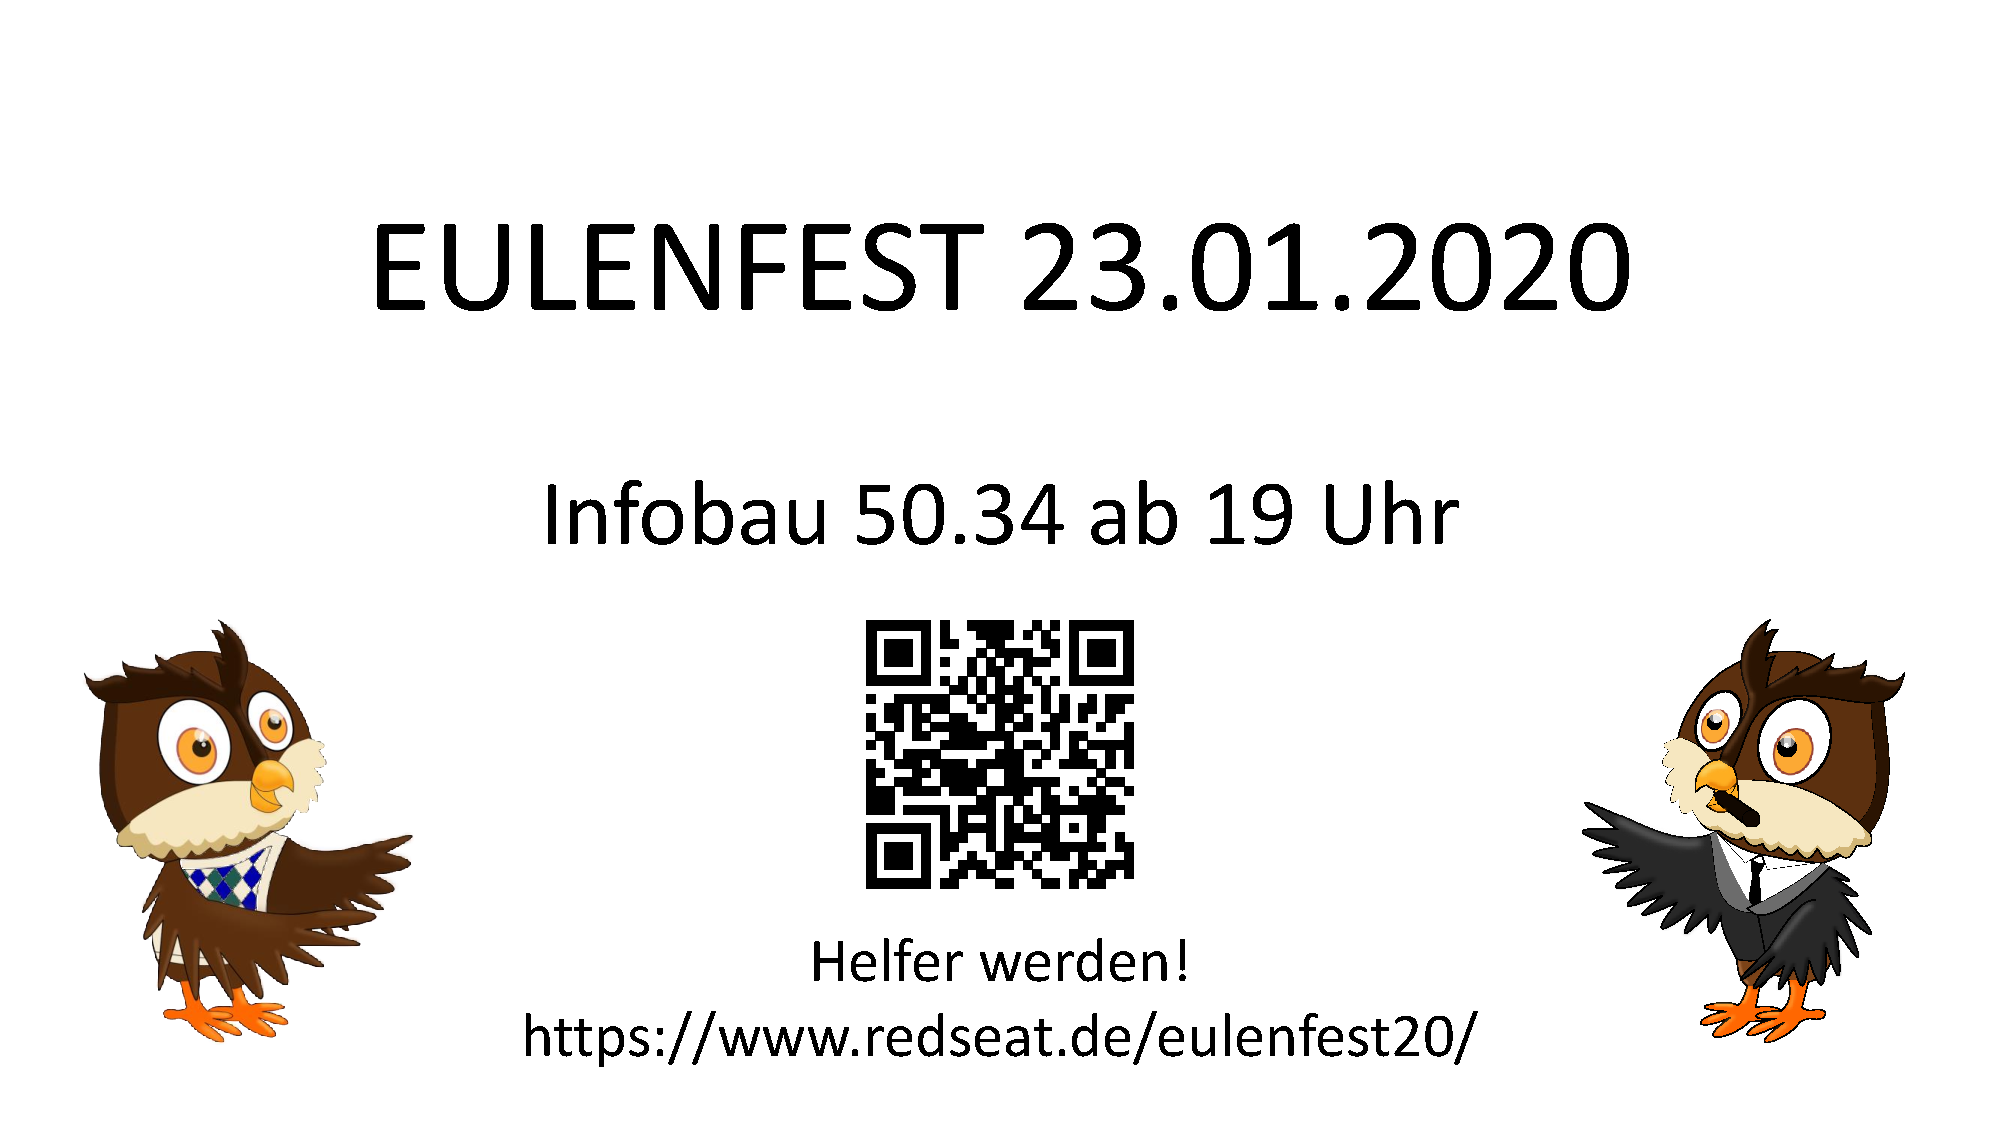
\includegraphics[width=1\textwidth]{../figures/EulenfestWerbung.pdf}
\questionframe
\lastframe
\mode<handout>{\slideThanks}
\end{document}
